% ============================================================
%  CHAPITRE 4 — Section 5 : Augmentation par la prévision de profils
% ============================================================
%
% NOTE : la prévision LSTM reprend, en version condensée, l'article EnergyCon
% (LaTeX/EnergyCon26_v1). Clés de citation à fusionner. Les chiffres de
% robustesse au bruit proviennent de python_these/Robustesse/Prédictions
% (README + robustesse_bruit_prevision.txt) et les figures de prévision de
% python_these/Prédictions profils.
% ============================================================

\section{Augmentation par la prévision des profils de puissance}
\label{sec:prediction}

Les deux premiers leviers exploitaient l'état interne du système. Le troisième porte sur son environnement~: anticiper l'évolution de la production photovoltaïque et de la consommation pour préparer le système aux sollicitations à venir. Cette section présente d'abord le levier de décision alimenté par la prévision, puis l'outil de prévision, et enfin la robustesse de l'apport face à l'incertitude de prévision.

% ------------------------------------------------------------
\subsection{Pré-charge de la batterie}
\label{subsec:precharge}
% ------------------------------------------------------------

La stratégie RB2(Pred) augmente RB2 d'un unique levier piloté par la prévision~: la pré-charge de la batterie. Lorsque la prévision annonce un déficit net, consommation supérieure à la production, sur l'horizon proche, et que la batterie dispose d'une marge de charge, l'électrolyseur est coupé ($P_{\text{ELY-set}}=0$). Le surplus de production photovoltaïque courant, sinon dirigé vers la chaîne hydrogène, vient alors charger la batterie.

L'intérêt est énergétique. Le stockage temporaire dans la batterie présente un rendement aller-retour de l'ordre de $95\,\%$, tandis que le stockage dans la chaîne hydrogène cumule les rendements de l'électrolyse et de la pile à combustible, de l'ordre de $0{,}7 \times 0{,}5$. En pré-chargeant la batterie avant un creux de production anticipé, le système aborde ce creux avec une réserve de SoC accrue, ce qui réduit les passages au plancher de charge et donc les pertes d'alimentation, sans surcoût de dégradation puisque la pré-charge redirige un surplus existant.

La grandeur de décision est l'énergie nette prévue, cumulée sur l'horizon de pré-charge $H_{\text{pre}}$~:
\begin{equation}
\label{eq:net_energy}
E_{\text{net}}(t) = \sum_{k=1}^{H_{\text{pre}}} \hat{P}_{\text{net}}(t+k)\,\Delta t,
\qquad
\hat{P}_{\text{net}} = \hat{P}_{\text{Load}} - \hat{P}_{\text{PV}},
\end{equation}
la pré-charge étant déclenchée lorsqu'un déficit net est prévu ($E_{\text{net}}>0$). Un balayage sur 25~ans a fixé l'horizon à $H_{\text{pre}}=\SI{18}{\hour}$, soit l'échelle diurne du système. Le déclenchement le plus performant est large, dès qu'un déficit net est prévu, plutôt que conditionné finement à l'état de la batterie.

RB2(Pred) ne diffère de RB2 que par une fonction de la prévision. Si la prévision est neutre, aucun déficit annoncé, ou désactivée, la stratégie retombe sur RB2. Tout gain est donc attribuable à la prévision. La pré-charge est ici greffée sur le meilleur RB2 statique (socle cost-min $0{,}440/0{,}310$, coût total $80{,}11$~k€), de sorte que le gain mesuré est celui d'une pré-charge sur un socle \emph{déjà optimisé}. Évalué avec une prévision omnisciente, le futur exact étant connu, le levier apporte un gain de $1{,}08$~k€ sur le coût total, de $80{,}11$~k€ à $79{,}03$~k€ (indicateur unifié VoLL $=3$~€/kWh). Ce gain est porté par la fiabilité, la LPSP passant de $2{,}59\,\%$ à $2{,}42\,\%$, la dégradation restant quasi inchangée. Cette valeur constitue une borne supérieure non atteignable, le vrai futur n'étant pas connu en exploitation.

% ------------------------------------------------------------
\subsection{Prévision par réseau LSTM}
\label{subsec:lstm}
% ------------------------------------------------------------

L'outil de prévision est un réseau récurrent à mémoire courte et longue (LSTM), dans la continuité de l'architecture développée au chapitre consacré au pronostic d'état de santé, ce qui illustre son caractère d'outil généraliste applicable aussi bien à l'extrapolation de SoH qu'à la prévision de profils de puissance. Les données sont des séries temporelles horaires de production PV et de consommation sur une année (\num{8760} points), exprimées en kW.

La chaîne de traitement suit des étapes classiques~: normalisation min-max des séries dans $[0,1]$, mise en forme par fenêtre glissante en tenseurs $[\text{échantillons}, \text{pas de temps}, \text{variables}]$, entraînement par rétropropagation avec l'optimiseur Adam et régularisation par \textit{dropout}, puis évaluation sur un jeu de test non vu à l'entraînement. La prévision multi-pas est obtenue de façon récursive, chaque sortie étant réinjectée en entrée pour le pas suivant, ce qui fait s'accumuler l'erreur sur l'horizon. Le partitionnement est chronologique, garantissant qu'aucune information postérieure à la séquence cible n'est utilisée. Les principaux hyperparamètres sont rassemblés au Tableau~\ref{tab:hyperparameters_ch4}.

\begin{table}[h!]
    \centering
    \caption{Hyperparamètres du réseau LSTM retenus pour la prévision PV et consommation.}
    \label{tab:hyperparameters_ch4}
    \begin{tabular}{lcc}
        \hline
        \textbf{Hyperparamètre} & \textbf{Valeur retenue} & \textbf{Plage explorée} \\
        \hline
        Taux d'apprentissage      & $10^{-3}$ & $[10^{-4},10^{-1}]$ \\
        Nombre d'unités LSTM      & $80$      & $[32,100]$          \\
        Taille de fenêtre         & $96$      & $[24,144]$          \\
        Nombre d'époques          & $160$     & $[20,200]$          \\
        \hline
    \end{tabular}
\end{table}

Les deux modèles, un par signal, reproduisent la structure temporelle de leurs séries respectives (Figure~\ref{fig:lstm_test}). Sur l'horizon de test de quatre jours, en prévision récursive multi-pas, le modèle de consommation atteint une RMSE de $0{,}380$~kW et le modèle PV une RMSE de $4{,}383$~kW. Le modèle PV capture l'enveloppe journalière de production, nulle la nuit et en cloche le jour, mais tend à produire un profil régulier d'un jour à l'autre et manque la variabilité météorologique fine. Cette limite reste sans conséquence majeure pour le levier de pré-charge, qui ne lit que le signe du bilan net cumulé.

\begin{figure}[h!]
    \centering
    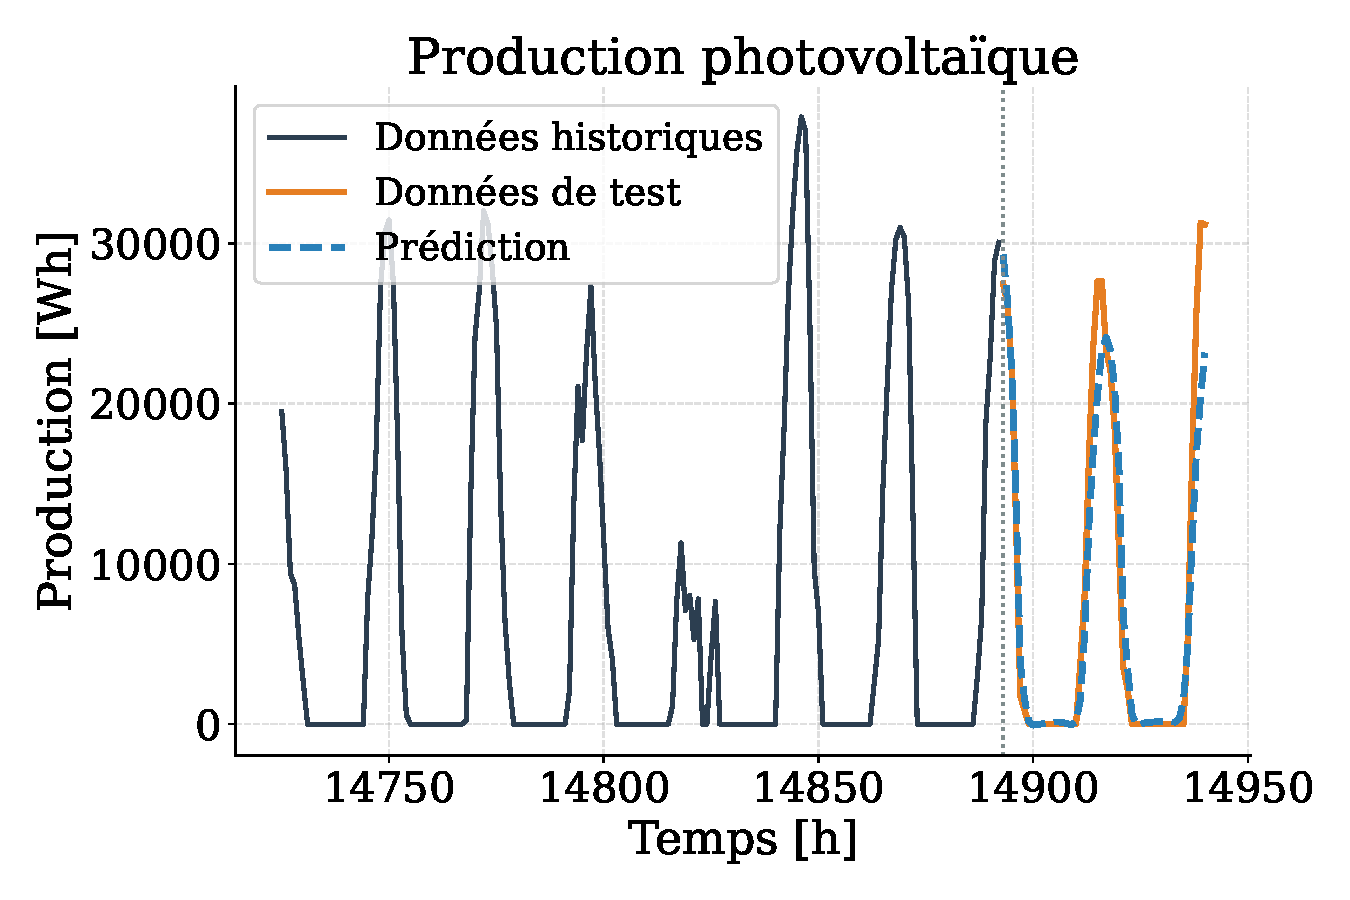
\includegraphics[width=.49\linewidth]{Chapitre 3/Prediction/Figures/lstm_pv.pdf}
    \hfill
    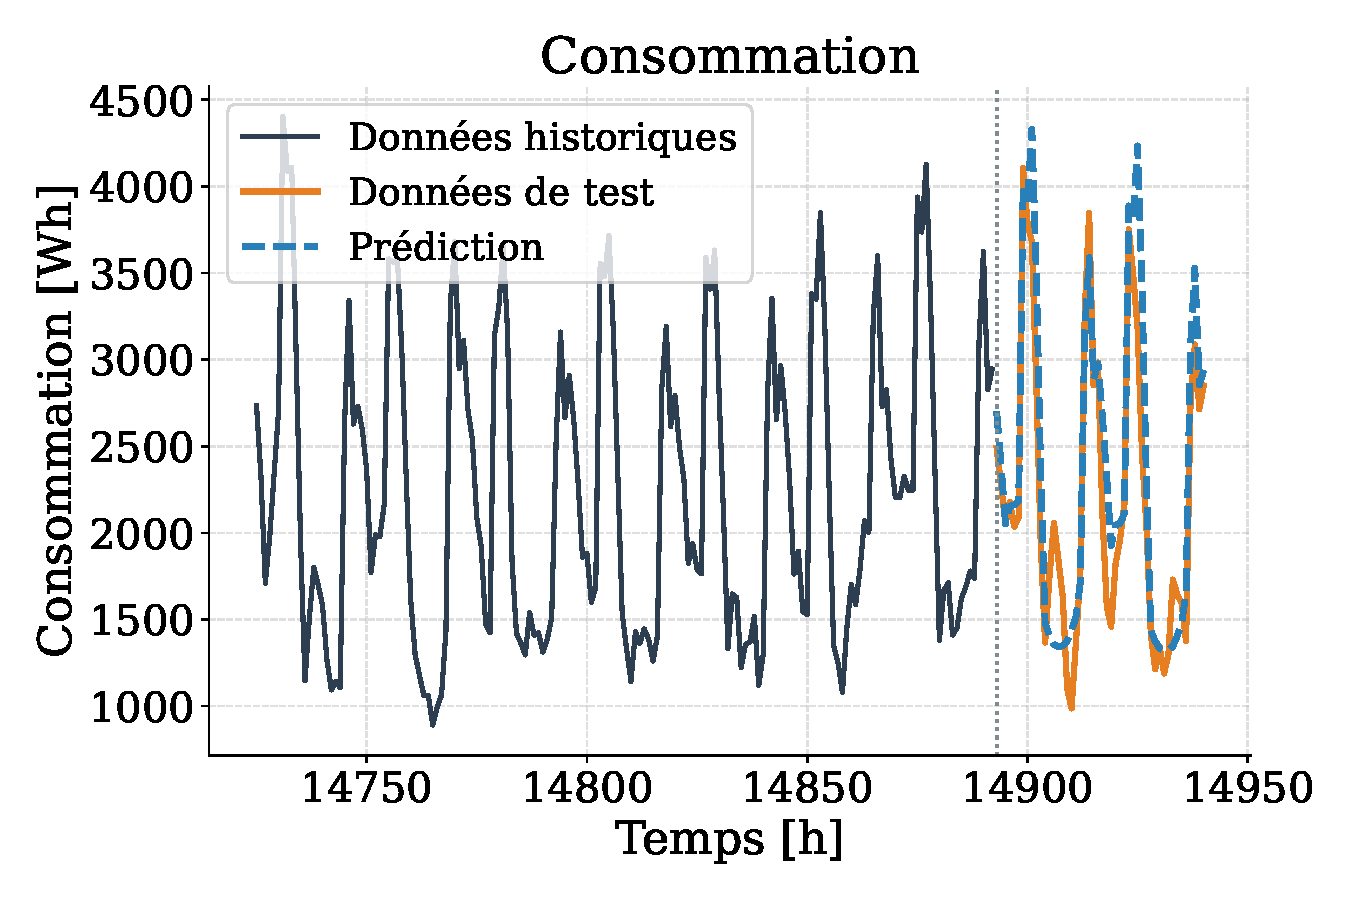
\includegraphics[width=.49\linewidth]{Chapitre 3/Prediction/Figures/lstm_load.pdf}
    \caption{Prévision récursive multi-pas sur le jeu de test~: modèle PV (gauche) et modèle consommation (droite).}
    \label{fig:lstm_test}
\end{figure}
\FloatBarrier

L'incertitude des prévisions a été estimée par \textit{Monte-Carlo Dropout}, en conservant le \textit{dropout} actif à l'inférence pour générer un ensemble de prédictions (Figure~\ref{fig:mc_dropout}). L'intervalle de prédiction est plus large pour la production PV que pour la consommation, conformément à la plus grande variabilité du signal solaire.

\begin{figure}[h!]
    \centering
    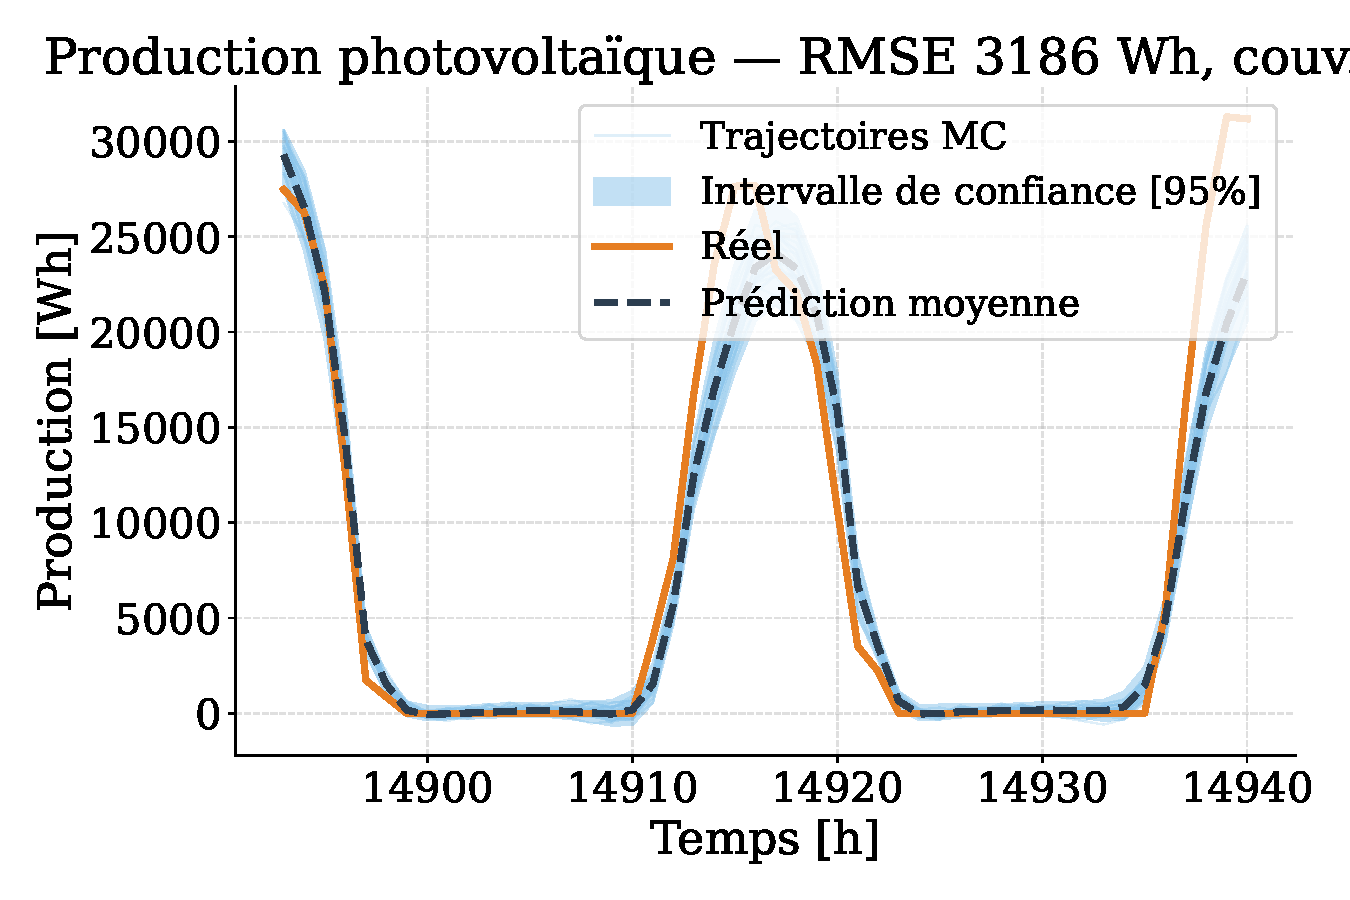
\includegraphics[width=.49\linewidth]{Chapitre 3/Prediction/Figures/pred_mcdropout_pv.pdf}
    \hfill
    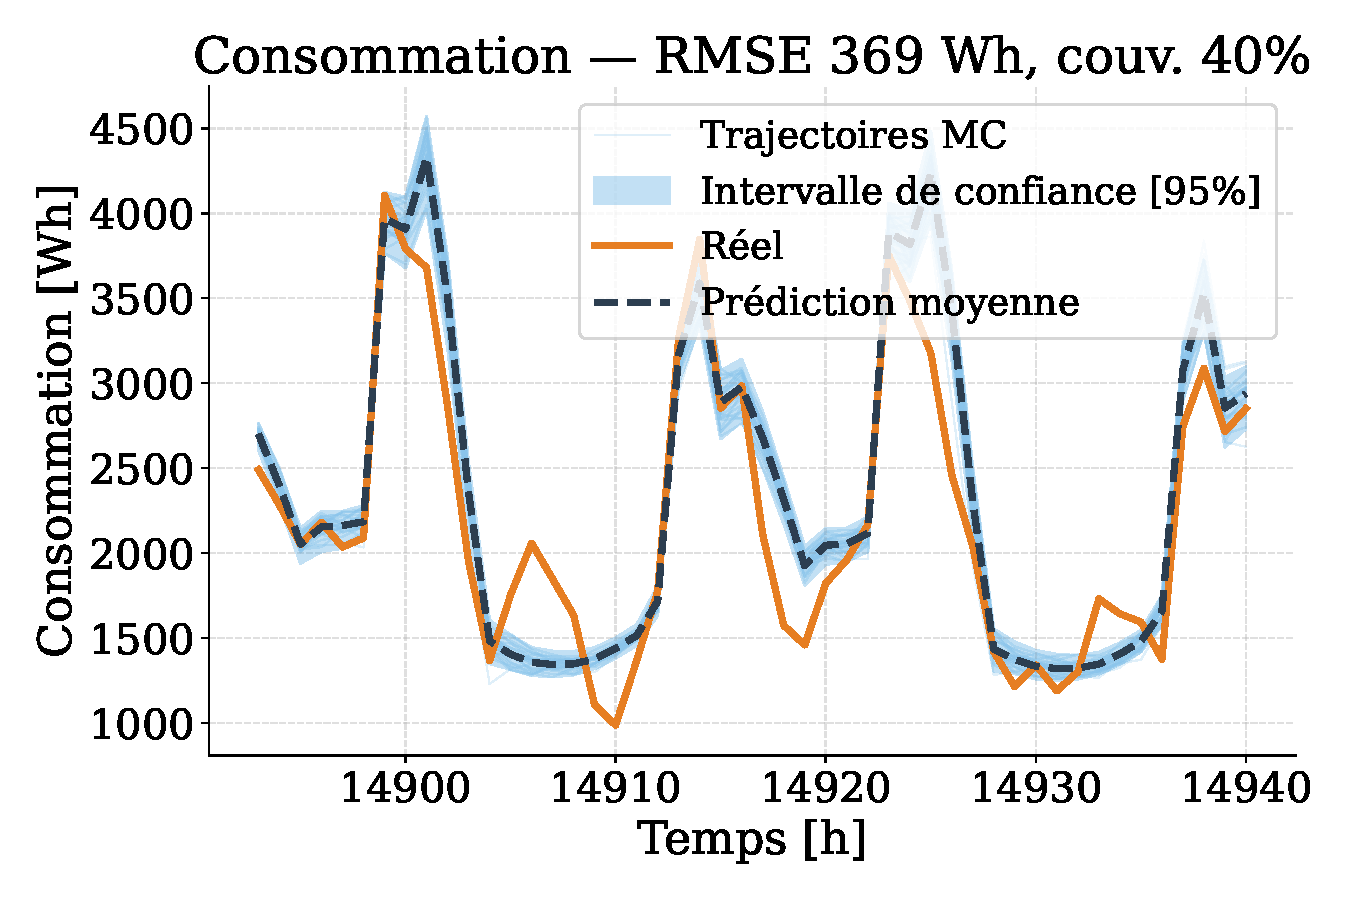
\includegraphics[width=.49\linewidth]{Chapitre 3/Prediction/Figures/pred_mcdropout_load.pdf}
    \caption{Intervalles de prédiction par Monte-Carlo Dropout~: production PV (gauche) et consommation (droite).}
    \label{fig:mc_dropout}
\end{figure}
\FloatBarrier

% ------------------------------------------------------------
\subsection{Incertitude de prévision}
\label{subsec:uncertainty}
% ------------------------------------------------------------

La pré-charge ne lit pas le profil détaillé, mais une seule grandeur scalaire~: l'énergie nette cumulée sur $H_{\text{pre}}=\SI{18}{\hour}$. C'est l'incertitude sur cette grandeur qu'il faut caractériser, et non la RMSE point par point. Un \textit{backtest} multi-origines (\num{216} origines du jeu de test) a permis de mesurer l'écart entre énergie nette prévue et énergie nette réelle (Figure~\ref{fig:net_uncertainty}). La distribution obtenue est quasi gaussienne, et à l'horizon de décision~:
\begin{equation}
\label{eq:noise_model}
E_{\text{net}}^{\text{prév}} = E_{\text{net}}^{\text{vrai}} + \mathcal{N}(\mu, \sigma),
\qquad \mu \approx \SI{-2.3}{\kilo\watt\hour}, \quad \sigma \approx \SI{39.4}{\kilo\watt\hour} \;\,(H_{\text{pre}}=\SI{18}{\hour}).
\end{equation}
Le biais est négligeable, l'écart-type substantiel. Ce $\sigma$ est mesuré contre la réalité~: il est irréductible. Il ne peut pas être réduit en moyennant davantage d'échantillons du modèle, le backtest utilisant déjà la prévision moyenne. À titre de repère, à \SI{48}{\hour} l'écart-type monte à environ \SI{80}{\kilo\watt\hour}~; sa valeur plus faible à \SI{18}{\hour} traduit la compensation partielle des erreurs horaires sur un horizon plus court.

\begin{figure}[h!]
    \centering
    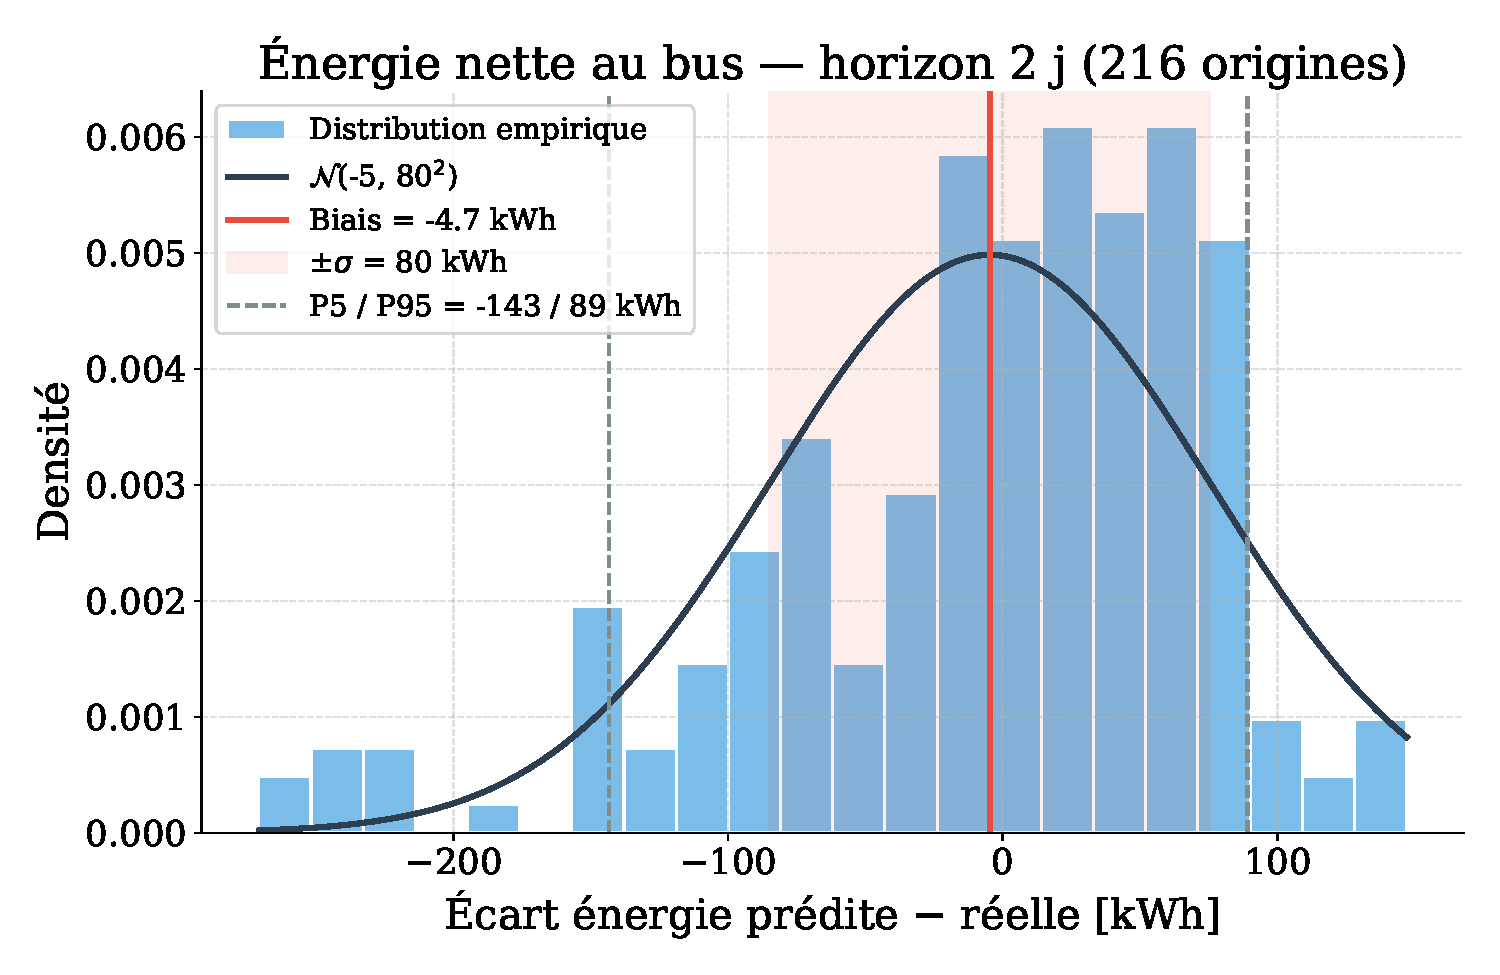
\includegraphics[width=.49\linewidth]{Chapitre 3/Prediction/Figures/pred_net_uncertainty.pdf}
    \hfill
    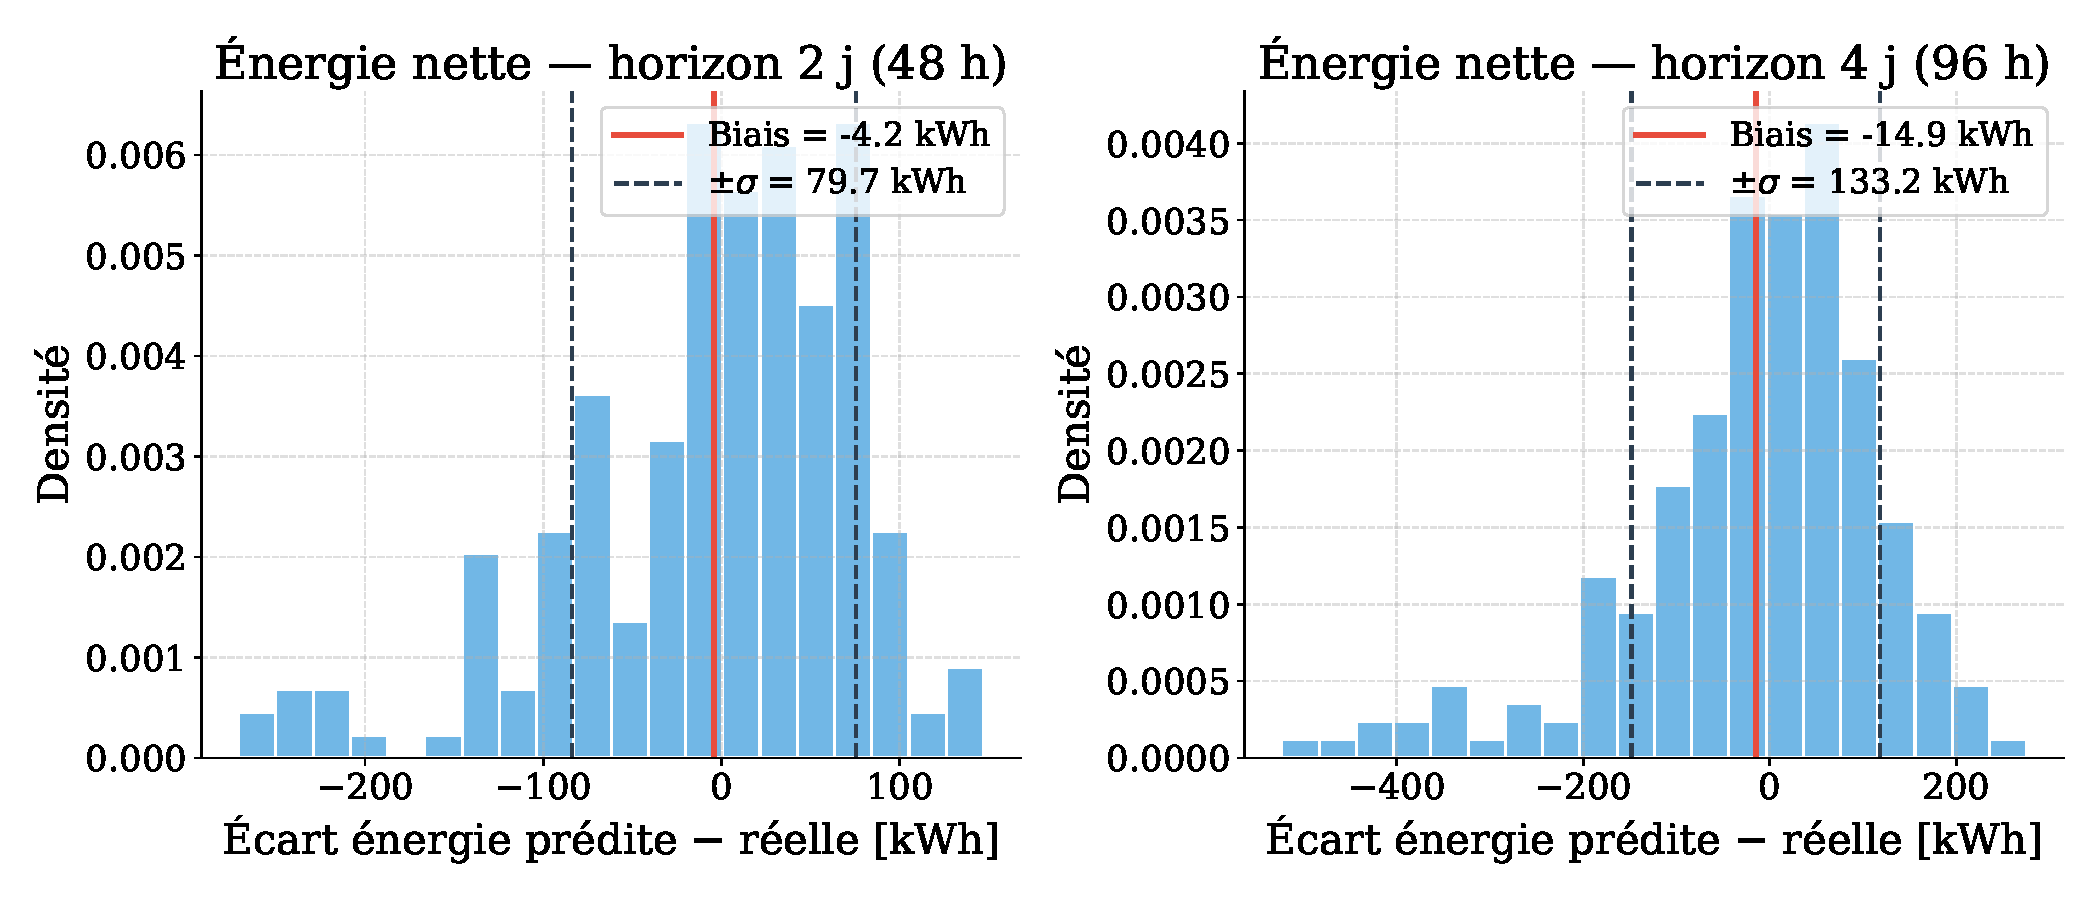
\includegraphics[width=.49\linewidth]{Chapitre 3/Prediction/Figures/pred_noise_distribution.pdf}
    \caption{Incertitude sur l'énergie nette prévue~: trajectoire prévue et réelle (gauche) et distribution de l'écart prévu-réel à l'horizon de décision (droite).}
    \label{fig:net_uncertainty}
\end{figure}
\FloatBarrier

% ------------------------------------------------------------
\subsection{Effet du bruit de prévision}
\label{subsec:fragility}
% ------------------------------------------------------------

\emph{Nota.} La caractérisation du bruit puis de l'hystérésis présentée dans cette sous-section et la suivante a été établie sur la base de référence (RB2 nominal, coût total $85{,}55$~k€), en amont de la ré-optimisation du socle de RB2. Elle démontre le \emph{mécanisme} de fragilité de la décision binaire puis de sa robustification, dont les conclusions qualitatives sont indépendantes du socle. Le point de fonctionnement robuste ré-basé sur le socle optimisé ($79{,}72$~k€) est reporté au Tableau~\ref{tab:soh_pred} et à la Figure~\ref{fig:pareto_rb2pred}~; la ré-exécution de ces balayages sur le socle ré-optimisé reste à mener.

En injectant le bruit réaliste~\eqref{eq:noise_model} dans la grandeur de décision, et en conservant la décision binaire d'origine, pré-charger si $E_{\text{net}}^{\text{prév}}>0$, le gain s'effondre (Tableau~\ref{tab:fragility}).

\begin{table}[h!]
\centering
\caption{Effet du bruit de prévision sur la pré-charge binaire (Monte-Carlo, 25~ans, coût total VoLL $=3$~€/kWh).}
\label{tab:fragility}
\begin{tabular}{lccc}
\hline
Variante & Coût total [k€] & LPSP [\%] & Démarrages ELY \\
\hline
RB2 (référence)                 & 85,55 & 2,454 & --- \\
RB2(Pred) omniscient (borne)    & 83,49 & 2,228 & 8961 \\
RB2(Pred) bruité, binaire       & 85,88 & 2,393 & 9736 \\
\hline
\end{tabular}
\end{table}

Le gain de $2{,}06$~k€ devient une perte de $0{,}33$~k€~: sous bruit réaliste, la pré-charge binaire fait pire que l'absence de prévision. Le surcoût de $2{,}39$~k€ par rapport à l'omniscient se décompose en environ $1{,}35$~k€ de LPSP, la pré-charge se déclenchant au mauvais moment, et $1{,}03$~k€ de dégradation.

Cette hausse de la dégradation s'explique par la nature binaire de la décision. Au voisinage du seuil $E_{\text{net}} \approx 0$, le bruit fait basculer la décision d'un pas de temps à l'autre, et l'électrolyseur clignote, ce qui engendre une dégradation de type démarrage-arrêt. Le décompte des démarrages de l'électrolyseur le confirme~: \num{8961} en omniscient contre \num{9736} sous bruit binaire, soit \num{775} démarrages parasites.

% ------------------------------------------------------------
\subsection{Robustesse par hystérésis}
\label{subsec:hysteresis}
% ------------------------------------------------------------

Le bruit étant irréductible, la décision est rendue tolérante au bruit en utilisant le $\sigma$ mesuré. Le seuil binaire est remplacé par une hystérésis à deux seuils sur l'énergie nette prévue, assortie d'une durée minimale de maintien~:
\begin{itemize}
  \setlength\itemsep{1pt}
  \item entrée en pré-charge, électrolyseur coupé, si $E_{\text{net}}^{\text{prév}} > +M_\sigma\,\sigma$~;
  \item sortie, électrolyseur rallumé, si $E_{\text{net}}^{\text{prév}} < -M_\sigma\,\sigma$~;
  \item entre les deux seuils, l'état courant est conservé, cette zone morte rejetant le bruit~;
  \item après chaque bascule, l'état est gelé pendant $T_{\text{dwell}}$ pas de temps, ce qui borne la fréquence de clignotement.
\end{itemize}
La demi-largeur de bande $\pm M_\sigma\,\sigma$ se cale sur l'incertitude quantifiée. Un balayage de Monte-Carlo sur $(M_\sigma, T_{\text{dwell}})$ a permis d'en régler les paramètres (Tableau~\ref{tab:hyst_sweep}).

\begin{table}[h!]
\centering
\caption{Balayage des paramètres d'hystérésis (Monte-Carlo 25~ans, moyenne sur 16 graines).}
\label{tab:hyst_sweep}
\begin{tabular}{cccccc}
\hline
$M_\sigma$ & $T_{\text{dwell}}$ [h] & Coût total [k€] & LPSP [\%] & Dégrad. [k€] & Démarrages ELY \\
\hline
0,50 & 0  & 84,83 & 2,336 & 65,68 & 9319 \\
0,50 & 12 & 84,58 & 2,379 & 65,07 & 9098 \\
1,00 & 0  & 84,51 & 2,334 & 65,36 & 9118 \\
1,00 & 6  & 84,49 & 2,349 & 65,23 & 9080 \\
\textbf{1,00} & \textbf{12} & \textbf{84,11} & \textbf{2,330} & \textbf{65,00} & \textbf{8976} \\
1,50 & 0  & 84,63 & 2,356 & 65,31 & 9075 \\
1,50 & 12 & 84,37 & 2,347 & 65,12 & 9003 \\
\hline
\end{tabular}
\end{table}

L'optimum est obtenu pour $M_\sigma=1{,}0$ et $T_{\text{dwell}}=\SI{12}{\hour}$~: le coût total descend à $84{,}11$~k€, soit un gain de $1{,}44$~k€ par rapport à RB2, et le clignotement de l'électrolyseur revient à son niveau omniscient (\num{8976} démarrages). L'hystérésis récupère ainsi environ $71\,\%$ du gain omniscient sous bruit réaliste (Tableau~\ref{tab:robust_summary}).

\begin{table}[h!]
\centering
\caption{Synthèse de la borne omnisciente au levier robuste (coût total).}
\label{tab:robust_summary}
\begin{tabular}{lcc}
\hline
Variante & Coût total [k€] & vs RB2 \\
\hline
RB2                                 & 85,55 & --- \\
RB2(Pred) omniscient (borne sup.)   & 83,49 & $-2{,}06$ \\
RB2(Pred) bruité, binaire           & 85,88 & $+0{,}33$ \\
RB2(Pred) bruité + hystérésis       & 84,11 & $-1{,}44$ \\
\hline
\end{tabular}
\end{table}

La bande de marge $\pm\sigma$ porte l'essentiel de la robustesse, le gel temporel n'étant qu'un complément. Deux tests le montrent. Geler la décision sans bande de marge ($M_\sigma=0$) est contre-productif, jusqu'à $87{,}21$~k€ pour un maintien long, car on fige une décision toujours bruitée. La bande seule ($M_\sigma=1$, $T_{\text{dwell}}=0$) suffit à inverser le signe du résultat, $1{,}04$~k€ de gain, avec la plus faible variance. Ajouté à la bande, le gel apporte un supplément de $0{,}40$~k€ en supprimant le clignotement résiduel. Un maintien trop long nuit, la LPSP remontant lorsque la décision figée rate les vraies transitions~; l'optimum $T_{\text{dwell}}=\SI{12}{\hour}$ correspond à la demi-journée diurne du système.

L'hystérésis est un dispositif de robustesse au bruit, et non une amélioration inconditionnelle. Appliquée sans bruit, avec les mêmes paramètres, elle retombe sur RB2~: la bande $\pm\SI{39}{\kilo\watt\hour}$ est trop large pour le signal vrai, les déficits nets à \SI{18}{\hour} étant souvent inférieurs à \SI{39}{\kilo\watt\hour}, et bloque alors les vrais déclenchements. C'est le bruit qui, par effet de \textit{dithering}, abaisse le seuil effectif et laisse passer les bons déclenchements. L'hystérésis ne doit donc pas être présentée comme un meilleur EMS dans l'absolu, mais comme le moyen de préserver la valeur de la prévision face à son incertitude.

Le positionnement de la stratégie prévisionnelle robuste dans le plan de Pareto est reporté à la Figure~\ref{fig:pareto_rb2pred}. Contrairement aux leviers SoH et RUL, RB2(Pred) agit sur la fiabilité~: son point se déplace vers les faibles LPSP à coût de dégradation quasi constant, franchissant une droite d'iso-coût unifié plus basse que RB2.

\begin{figure}[h!]
    \centering
    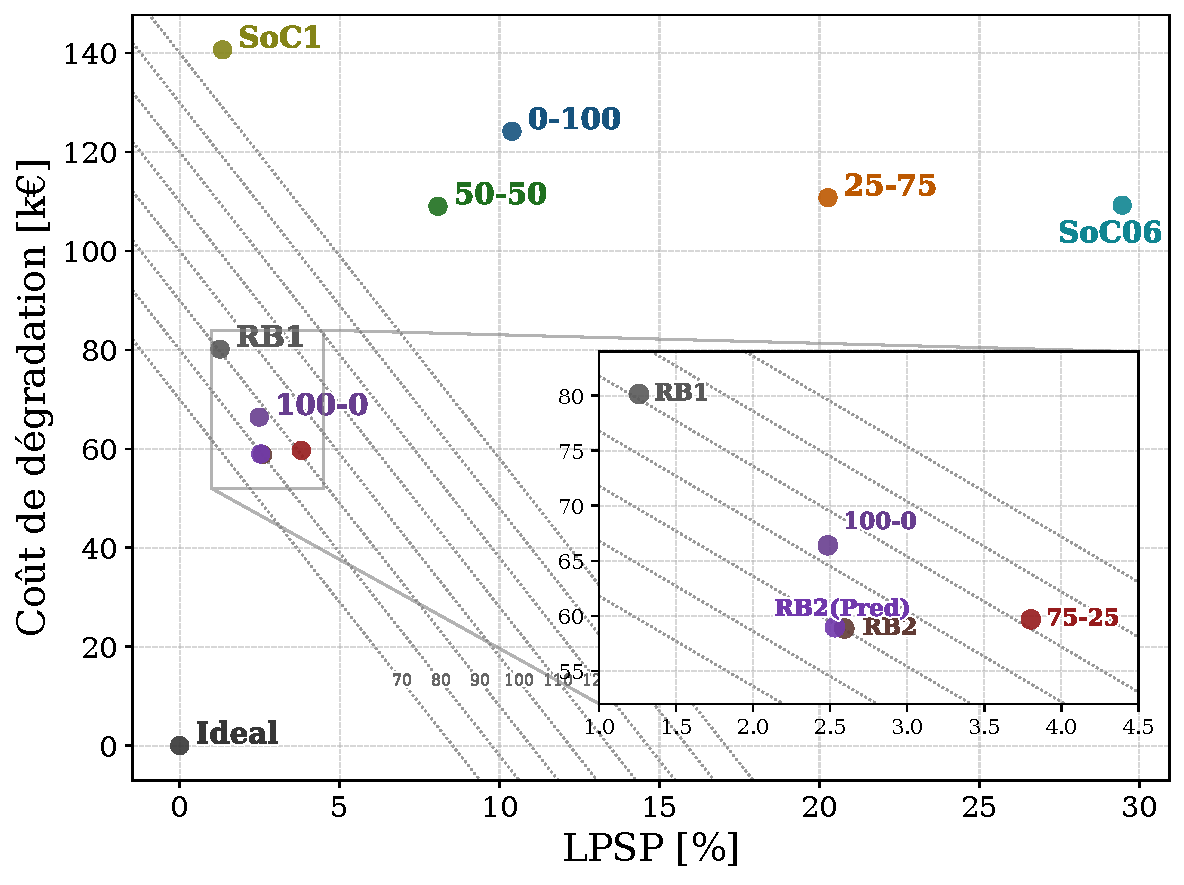
\includegraphics[width=\linewidth]{Chapitre 3/Prediction/Figures/pareto_pred_isocost.pdf}
    \caption{Positionnement de RB2(Pred) (variante hystérésis, Monte-Carlo) dans le plan de Pareto LPSP--coût de dégradation, parmi le panel du chapitre précédent (agrandissement sur l'amas RB2 en encart). Les droites pointillées grises sont les lignes d'iso-coût total unifié (dégradation $+$ valorisation de la LPSP à VoLL~$=3$~€/kWh, pente $8{,}2$~k€ par point de LPSP)~; leur étiquette donne le coût total en k€.}
    \label{fig:pareto_rb2pred}
\end{figure}
\FloatBarrier

Le bruit est supposé gaussien et indépendant d'un pas à l'autre, ce qui constitue le pire cas pour le clignotement~: des prévisions réelles consécutives, dont les fenêtres se recouvrent, seraient corrélées et engendreraient moins de clignotement. Une modélisation à bruit corrélé reste à explorer. Le $\sigma$ retenu est par ailleurs spécifique à l'horizon de décision, au jeu de données et au modèle LSTM courant.

% ------------------------------------------------------------
\subsection{Combinaison de l'état de santé et de la prévision}
\label{subsec:soh_pred}
% ------------------------------------------------------------

Les leviers SoH et prévision agissent sur des grandeurs différentes, durabilité pour le premier, fiabilité pour le second, et peuvent être combinés. La stratégie RB2(SoH+Pred) greffe la pré-charge robuste sur la base déjà augmentée par l'état de santé. Les performances, évaluées en Monte-Carlo (\num{200} tirages, 25~ans), sont reportées au Tableau~\ref{tab:soh_pred}.

\begin{table}[h!]
\centering
\caption{Stratégies combinées, sur socle optimisé (variante hystérésis, moyenne Monte-Carlo, 25~ans, VoLL~$=3$~€/kWh).}
\label{tab:soh_pred}
\begin{tabular}{lccc}
\hline
Stratégie & LPSP [\%] & Coût de dégradation [k€] & Coût total [k€] \\
\hline
RB2 (référence)   & 2,59 & 58,85 & 80,11 \\
RB2(SoH)          & 2,91 & 54,91 & 78,77 \\
RB2(Pred)         & 2,53 & 58,97 & 79,72 \\
RB2(SoH+Pred)     & 2,75 & 55,08 & 77,67 \\
\hline
\end{tabular}
\end{table}

RB2(Pred) améliore le coût total par rapport à RB2 ($80{,}11 \to 79{,}72$~k€), par une meilleure LPSP à dégradation quasi inchangée. RB2(SoH+Pred) gagne à son tour sur la LPSP par rapport à RB2(SoH), à dégradation quasi identique, et atteint le meilleur coût total du chapitre ($77{,}67$~k€)~: le levier de prévision se transfère sur la base augmentée par l'état de santé, ce qui confirme la complémentarité des deux connaissances. La dispersion Monte-Carlo de ces points est faible, l'écart-type de dégradation valant $0{,}04$ à $0{,}16$~k€~: sur l'agrégat de 25~ans, environ \num{219000} pas, le bruit horaire indépendant s'auto-moyenne et l'indicateur final est quasi déterministe.

Le positionnement de la stratégie combinée est reporté à la Figure~\ref{fig:pareto_sohpred}. RB2(SoH+Pred) réunit les deux déplacements~: le gain de durabilité apporté par l'état de santé (comme RB2(SoH)) et le gain de fiabilité apporté par la prévision (comme RB2(Pred)), aboutissant à la droite d'iso-coût unifié la plus basse de l'amas RB2.

\begin{figure}[h!]
    \centering
    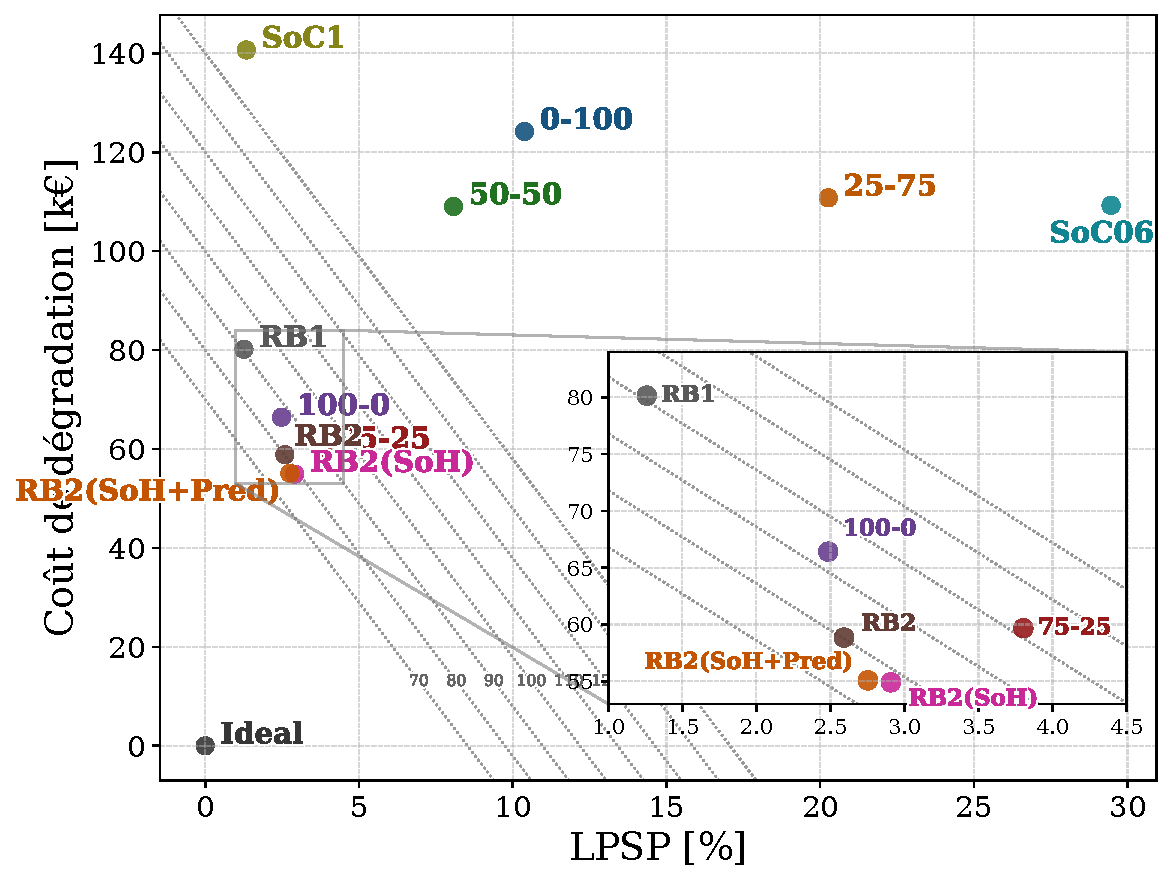
\includegraphics[width=\linewidth]{Chapitre 3/Prediction/Figures/pareto_sohpred_isocost.pdf}
    \caption{Positionnement de RB2(SoH+Pred) dans le plan de Pareto LPSP--coût de dégradation, avec RB2 et RB2(SoH), parmi le panel du chapitre précédent (agrandissement sur l'amas RB2 en encart). Les droites pointillées grises sont les lignes d'iso-coût total unifié (dégradation $+$ valorisation de la LPSP à VoLL~$=3$~€/kWh, pente $8{,}2$~k€ par point de LPSP)~; leur étiquette donne le coût total en k€.}
    \label{fig:pareto_sohpred}
\end{figure}
\FloatBarrier
